% !TeX root = Tesis.tex
% !TeX spellcheck = es
% !TeX encoding = UTF-8
\chapter{}
\label{apx:apx1}

\begin{figure}[!htb]
	\centering
	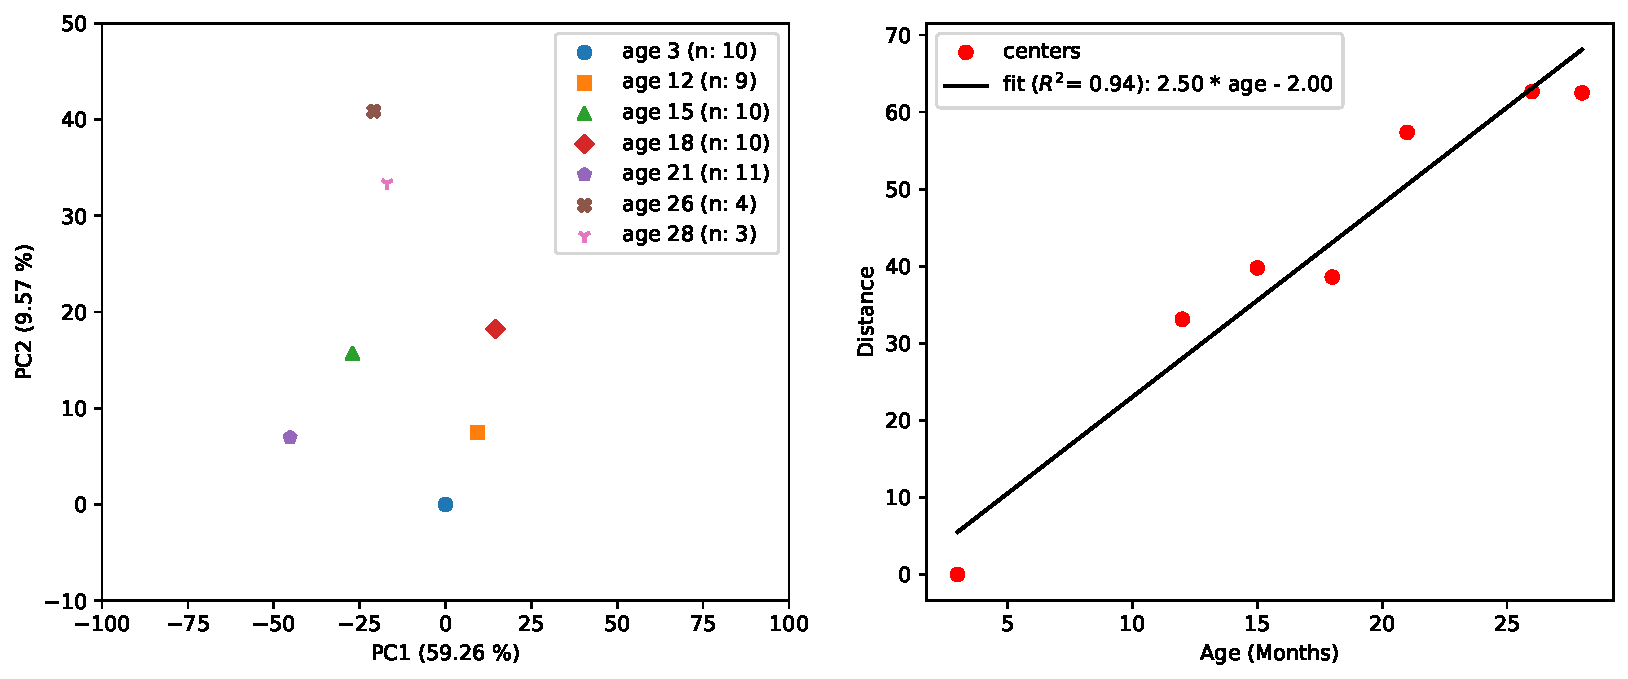
\includegraphics[width=\linewidth]{figures/suppl_fig_1}
	\caption{Representación gráfica de los datos de la referencia \cite{hahn2023atlas} en un modelo de ratón para el cuerpo calloso, una región rica en materia blanca.}
	\label{fig:suppl1}
\end{figure}

Panel izquierdo: Análisis de componentes principales de los datos. Se muestran los centros de los subgrupos de muestras. Se consideran edades entre 3 y 28 meses. Se observa una dirección de envejecimiento.

Panel derecho: Distancias completas (incluyendo todos los componentes) hasta el punto inicial (3 meses). Esta figura muestra que la proyección al plano (PC1, PC2) es una representación fiel.
